Nous venons donc de voir trois algorithmes de factorisation.\\
Le premier est celui des divisions successives qui, comme nous l’avons expliqué précédemment, est efficace
pour trouver de petits facteurs.\\
Le deuxième est la méthode de Fermat, il est lui efficace quand les facteurs sont proches. \\
Le dernier, celui du crible quadratique, est le plus efficace quel que soit le nombre.\\
Nous avons donc essayé de les comparer pour voir lequel de ces algorithmes est le meilleur. \\
Pour se faire, on a généré 100 nombres aléatoires entre $1$ et $10^{20}$, puis tenté de les factoriser successivement par les
trois algorithmes. Le temps pris pour factoriser chacun des chiffres est modélisé par un graphe généré en Python. \\

Voici le résultat :\\
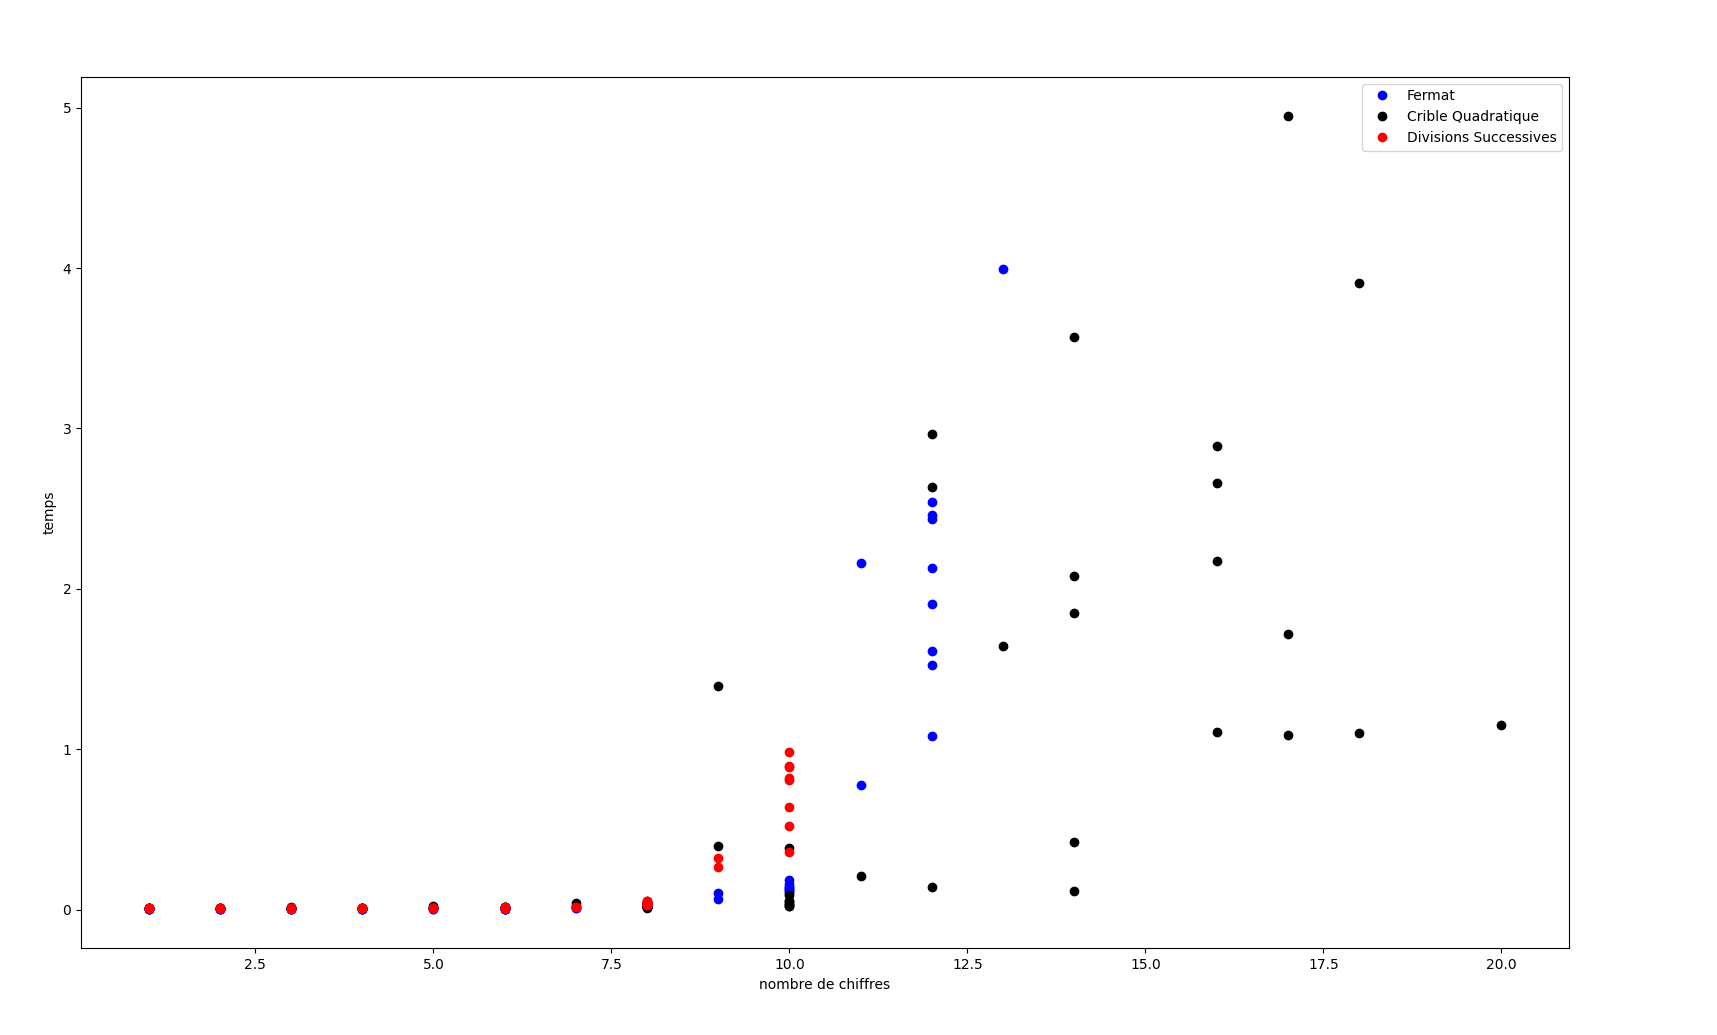
\includegraphics[width=0.75\textwidth]{media/4.png}\\
Si le temps de factorisation dépasse 5 secondes, on n’en tient pas compte et on passe au nombre suivant. \\
Ce graphe confirme nos prévisions : l’algorithme fondé sur le crible quadratique est le plus optimal. Il est en général plus rapide que les autres et il génère des solutions pour de plus grandes valeurs.
La méthode de Fermat est plus efficace que celle par divisions successives. Elle n'arrive cependant plus à factoriser à partir d’un nombre à 12 chiffres.La méthode par divisions successives quant a elle est la moins efficace. Elle échoue a factoriser un nombre s'il est supérieur à $10^{10}$.